\chapter{Аналитическая часть}

В данном разделе формально описывается процесс продажи вина. Изучаются и сравниваются существующие модели баз данных и системы управления базами данных. В результате анализа определяются модель базы данных и система управления базами данных, оптимальные для решения поставленной задачи.

\section{Формализация задачи}

Описать процесс продажи вина.

\section{Формализация ролей}

Участниками виноторговли являются поставщик вин и потребитель. Для управления их запросами в информационной системе необходим администратор.

Для поставщика определены следующие действия:

\begin{itemize}
	\item регистрация в системе;
	\item вход в аккаунт;
	\item выход из аккаунта;
	\item получение данных:
		\begin{itemize}
			\item о вине;
			\item о продажах;
		\end{itemize}		 
	\item создание запроса:
		\begin{itemize}
			\item на добавление нового товара;
			\item на удаление товара;
			\item на редактирование товара.
		\end{itemize}
\end{itemize}

В возможности потребителя входит:

\begin{itemize}
	\item регистрация в системе;
	\item вход в аккаунт;
	\item выход из аккаунта;
	\item получение данных:
		\begin{itemize}
			\item о вине;
			\item о поставщике;
			\item о рейтинге вин;
			\item о покупках;
		\end{itemize}
	\item создание запроса на получение бонусной карты.
\end{itemize}

Администратор обладает правами на следующие действия:

\begin{itemize}
	\item вход в аккаунт;
	\item выход из аккаунта;
	\item получение данных:
		\begin{itemize}
			\item о вине;
			\item о продажах;
		\end{itemize}
	\item одобрение или отклонение:
		\begin{itemize}
			\item выдачи бонусной карты пользователю;
			\item добавления товара поставщика;
			\item удаления товара поставщика;
			\item редактирования товара поставщика.
		\end{itemize}
\end{itemize}

\section{Формализация данных}

\section{Анализ БД}

\section{Анализ СУБД}

\section{Анализ существующих решений}

Под вопросом, если будет, то добавить про это во введение к разделу и вывод.

\section{Вывод}

\chapter{Конструкторская часть}

\begin{figure}[H]
	\begin{center}
		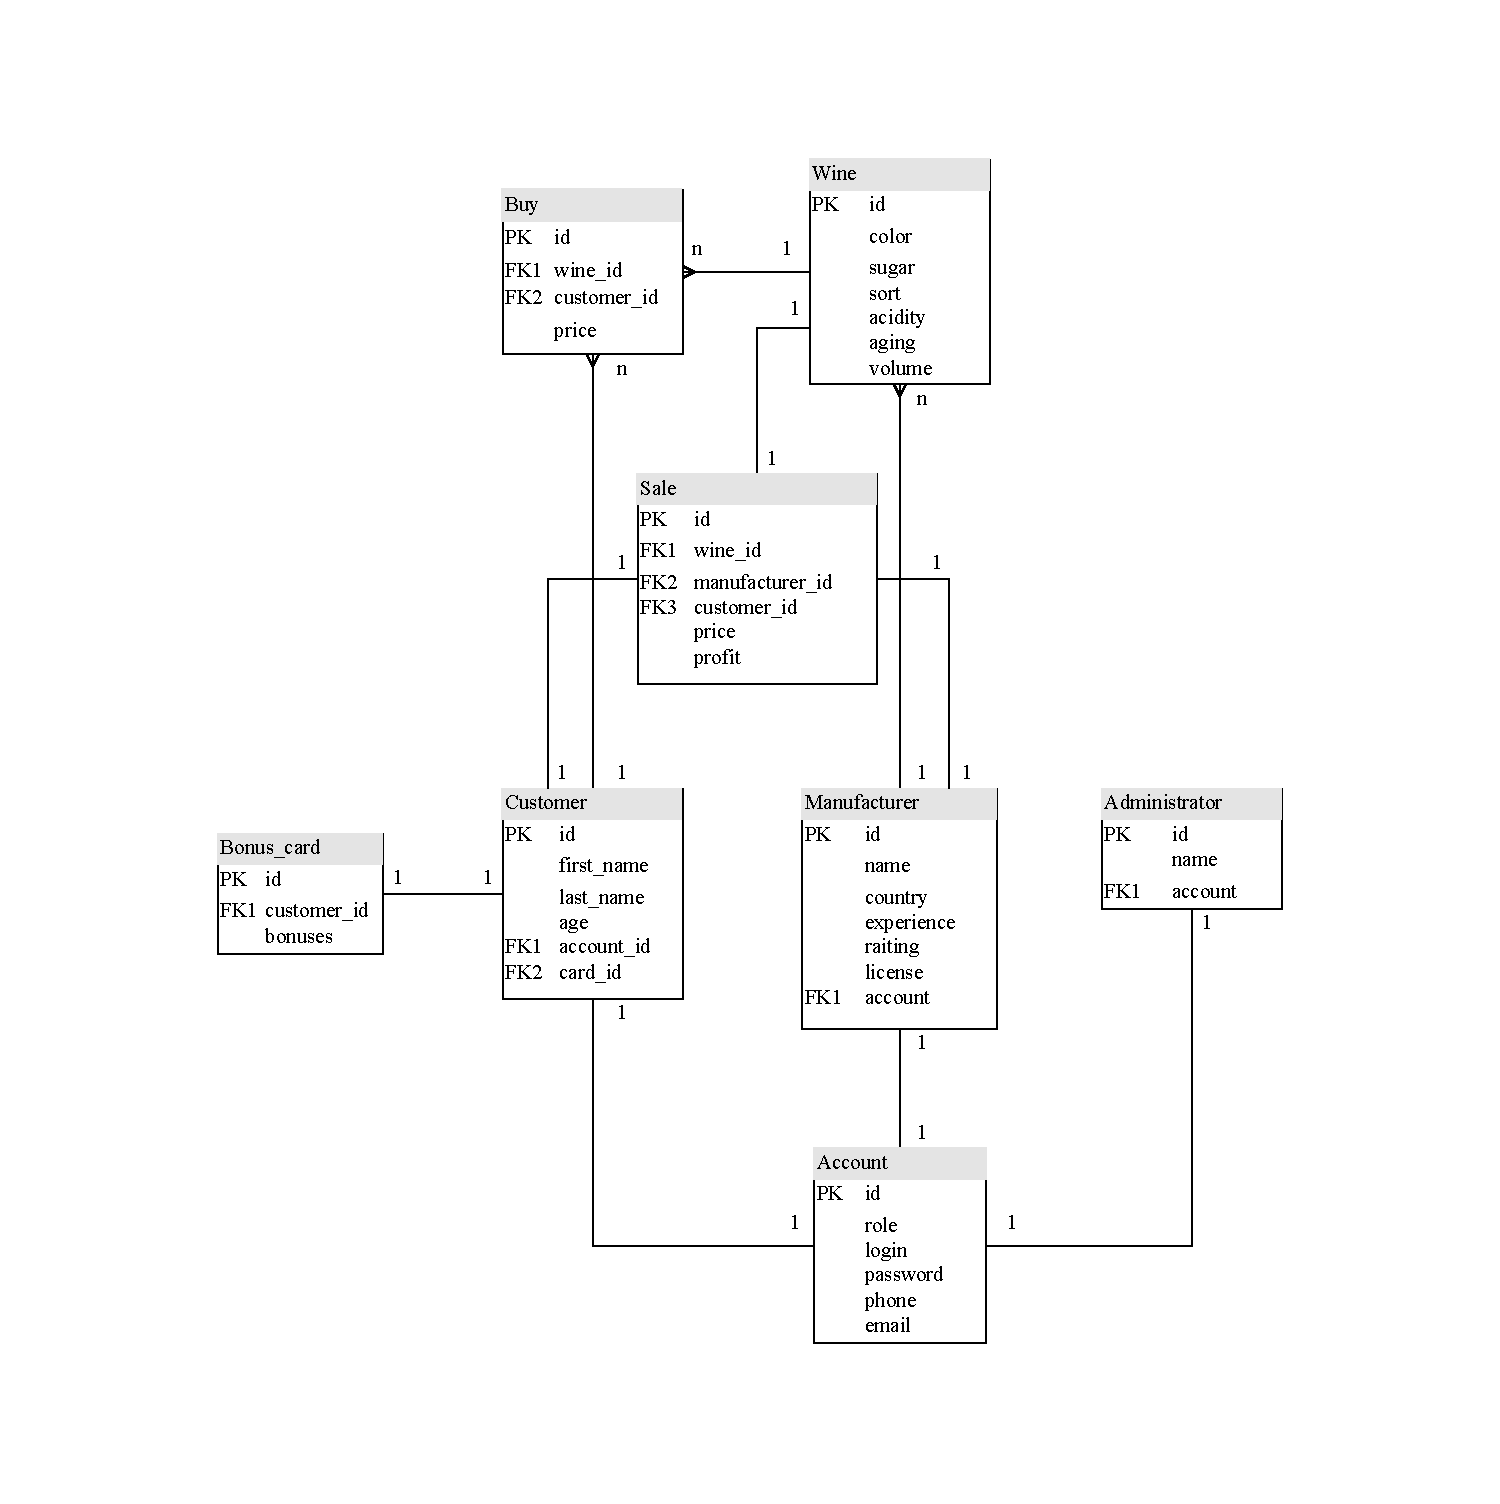
\includegraphics[scale=0.75]{img/ER-diagram.pdf}
	\end{center}
	\captionsetup{justification=centering}
	\caption{ER-диаграмма сущностей}
	\label{img:er}
\end{figure}

\section{Use-case диаграммы}

\begin{figure}[H]
	\begin{center}
		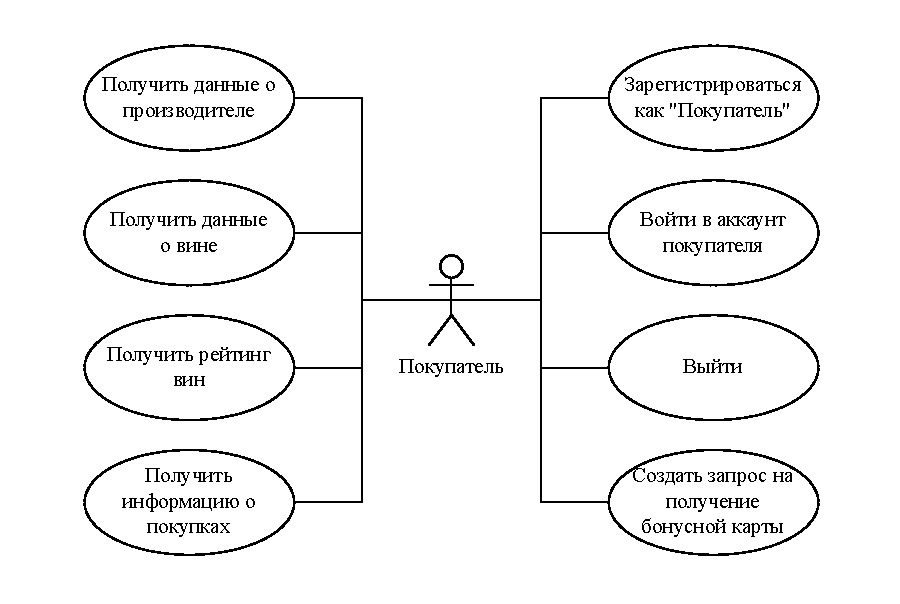
\includegraphics[scale=0.8]{img/customer.pdf}
	\end{center}
	\captionsetup{justification=centering}
	\caption{Use-case - покупатель}
	\label{img:customer}
\end{figure}

\begin{figure}[H]
	\begin{center}
		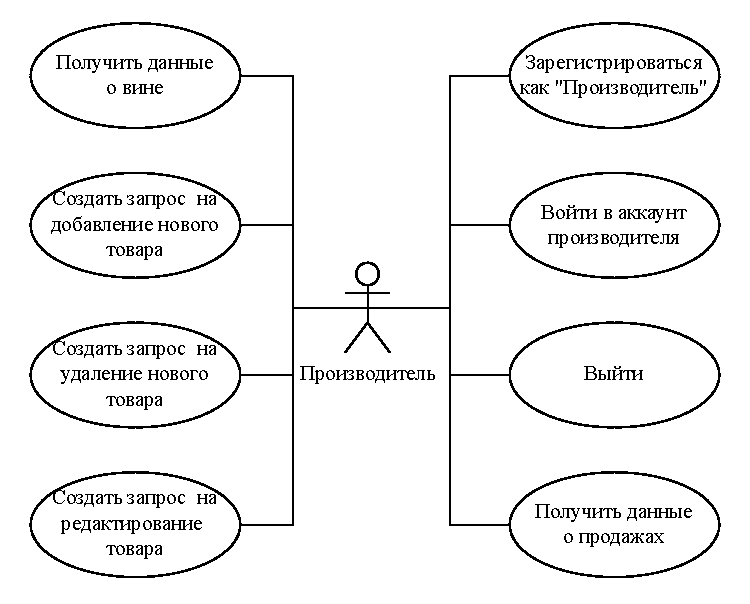
\includegraphics[scale=0.8]{img/manufacturer.pdf}
	\end{center}
	\captionsetup{justification=centering}
	\caption{Use-case - производитель}
	\label{img:manufacturer}
\end{figure}

\begin{figure}[H]
	\begin{center}
		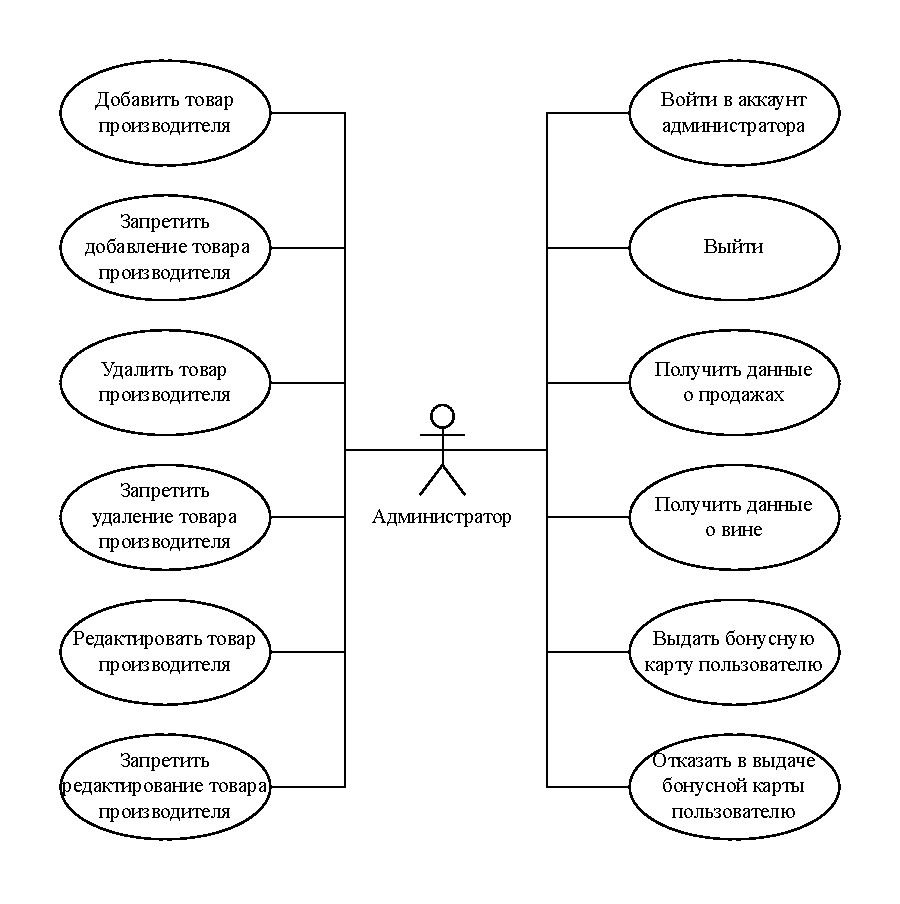
\includegraphics[scale=0.8]{img/administrator.pdf}
	\end{center}
	\captionsetup{justification=centering}
	\caption{Use-case - администратор}
	\label{img:administrator}
\end{figure}